
% Preamble
\documentclass[12pt, letterpaper]{article}
\title{Chapter 3 - Partial Differential Equations - Notes}
\author{Jordan Tucker}
\date{April 5, 2026}
% Packages
\usepackage{amsmath}
\usepackage{parskip}
\usepackage{tabularx}
\usepackage{graphicx}
\usepackage{hyperref} %LaTeX package to import graphics
\graphicspath{{images/}} %configuring the graphicx package

% Document
\begin{document}
    \maketitle
    \section{A Mathematical Representation of Waves}
    \subsection{Introduction and examples}
    If a function $u$ is the value of some measurement of a one dimensional medium that depends on
    position $x$ and time $t$,the partial derivatives of $u$ with respect to $x$ and $t$ have
    important physical meanings.

    A \textbf{partial differential equation} (PDE) for a function $u(x,t)$ is a differential equation that
    involves one or more of the partial derivatives of $u$ with respect to $x$ and $t$.
    We will usually denote the partial derivatives of $u$ by
    \[
    u_t = \frac{\partial u}{\partial t}, \quad u_x = \frac{\partial u}{\partial x}, \quad u_{xt} = \frac{\partial^2 u}{\partial t \partial x},\quad  \dots
    \]

    Common PDEs with solutions illustrating waves:
    \begin{enumerate}
        \item[(a)] Advection equation: $u_t+cu_x=0$.
        \item[(b)] Diffusion equation: $u_t=Du_{xx}$.
        \item[(c)] The linearized Burgers equation: $u_t+cu_x=Du_{xx}$.
        \item[(d)] Burgers equation: $u_t+uu_x=Du_{xx}$.
        \item[(e)] Inviscid Burgers equation: $u_t+uu_x=0$.
        \item[(f)] Wave equation: $u_{tt}=c^2 u_{xx}$.
        \item[(g)] Korteweg-deVries equation: $u_t+uu_x+u_{xxx}=0$.
    \end{enumerate}

    \subsection{An intuitive view}\label{subsec:an-intuitive-view}
    At a fixed position $x$ in the medium, the value of $u_t(x, t)$ gives the rate at which $u$ is
    changing with respect to time.
    A positive value of $u_t(x,t)$ indicates that at position $x$, $u$ is increasing as time
    increases.
    A negative value of $u_t(x,t)$ indicates that $u$ is decreasing at position $x$ as time
    increases.
    In applications where $u(x,t)$ denotes a displacement at position $x$, $u_t(x,t)$ and $u_{tt}(x,t)$
    have the particular interpretation of velocity and acceleration.

    At a fixed time t, the values of $u_x(x,t)$ and $u_{xx}(x,t)$ provide information about the
    slope and concavity of the graph of $u(x, t)$ as a function of $x$.
    In particular applications these represent quantities such as flux and stress.

    \textbf{Example:} Suppose $u$ represents the temperature on a rod at position $x$ and time $t$.
    Suppose the temperature of the rod is governed by the heat equation:
    \[
        u_t = Du_{xx} \quad (D>0\quad constant),
    \]
    $u_t$ is directly proportional to the concavity of $u(x,t)$.
    If $u(x,t)$ is concave up, $u_t$ is positive so the temperature will increase.
    If $u(x,t)$ is concave down, $u_t$ is negative so the temperature will decrease.
    This makes sense because heat flows from hotter regions to colder regions.
    \begin{figure}[h]
        \centering
        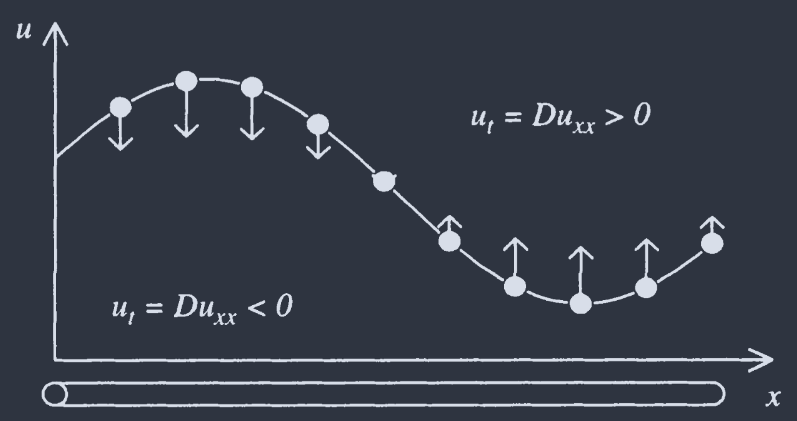
\includegraphics[width=0.75\textwidth]{heat}
        \caption{According to the heat equation, the change in temperature $u$ at each point $x$ depends on the concavity of the temperature profile at that instant.}\label{fig:figure}
    \end{figure}
    \newpage
    \subsection{Terminology}\label{subsec:terminology}
    PDEs can be classified many different ways.

    The \textbf{order} of a PDE is the order of the highest order partial derivative in PDE\@.

    A PDE is \textbf{first order linear} if it follows the form
    \begin{equation}
        a_1 u_t + a_2 u_x + bu = f\label{eq:equation}
    \end{equation}
    Where $a_1$ and $a_2$ are not both 0, and $a_1$, $a_2$, $b$, and $f$ are constants or functions
    of $x$ and $t$ (but cannot depend on $u$).
    If a first order PDE cannot be written in this form,
    then it is \textbf{nonlinear}.

    A PDE is \textbf{second order linear} if it can be written in the form
    \begin{equation}
        a_{11} u_{tt} + a_{12} u_{tx} + a_{22} u_{xx} + b_1 u_t + b_2 u_x + cu = f
    \end{equation}
    Where $a_{11}$, $a_{12}$, and $a_{22}$ are not all zero, and $a_{ij}$, $b_i$, $c$, and $f$ are
    constants or functions of $x$ and $t$ (but don't depend on $u$).
    If a second order PDE does not follow this form, then it is \textbf{non-linear}.

    We can typically classify linear equations and \textbf{homogeneous}.
    If $f=0$, then the PDE is \textbf{homogeneous}.
    If $f\neq0$, then the PDE is \textbf{nonhomogeneous}.
    We typically do not classify nonlinear PDEs as homogeneous or nonhomogeneous.

\end{document}